\chapter{Application setup}\label{appendix:setup}

\figref{fig:setup} shows the setup that we have made on the \theinstitute's
machines (not all connections between \code{mongos} and \code{mongod} instances
are shown). Client, Server and Scraper use this configuration by default.

\begin{figure}[htb]
	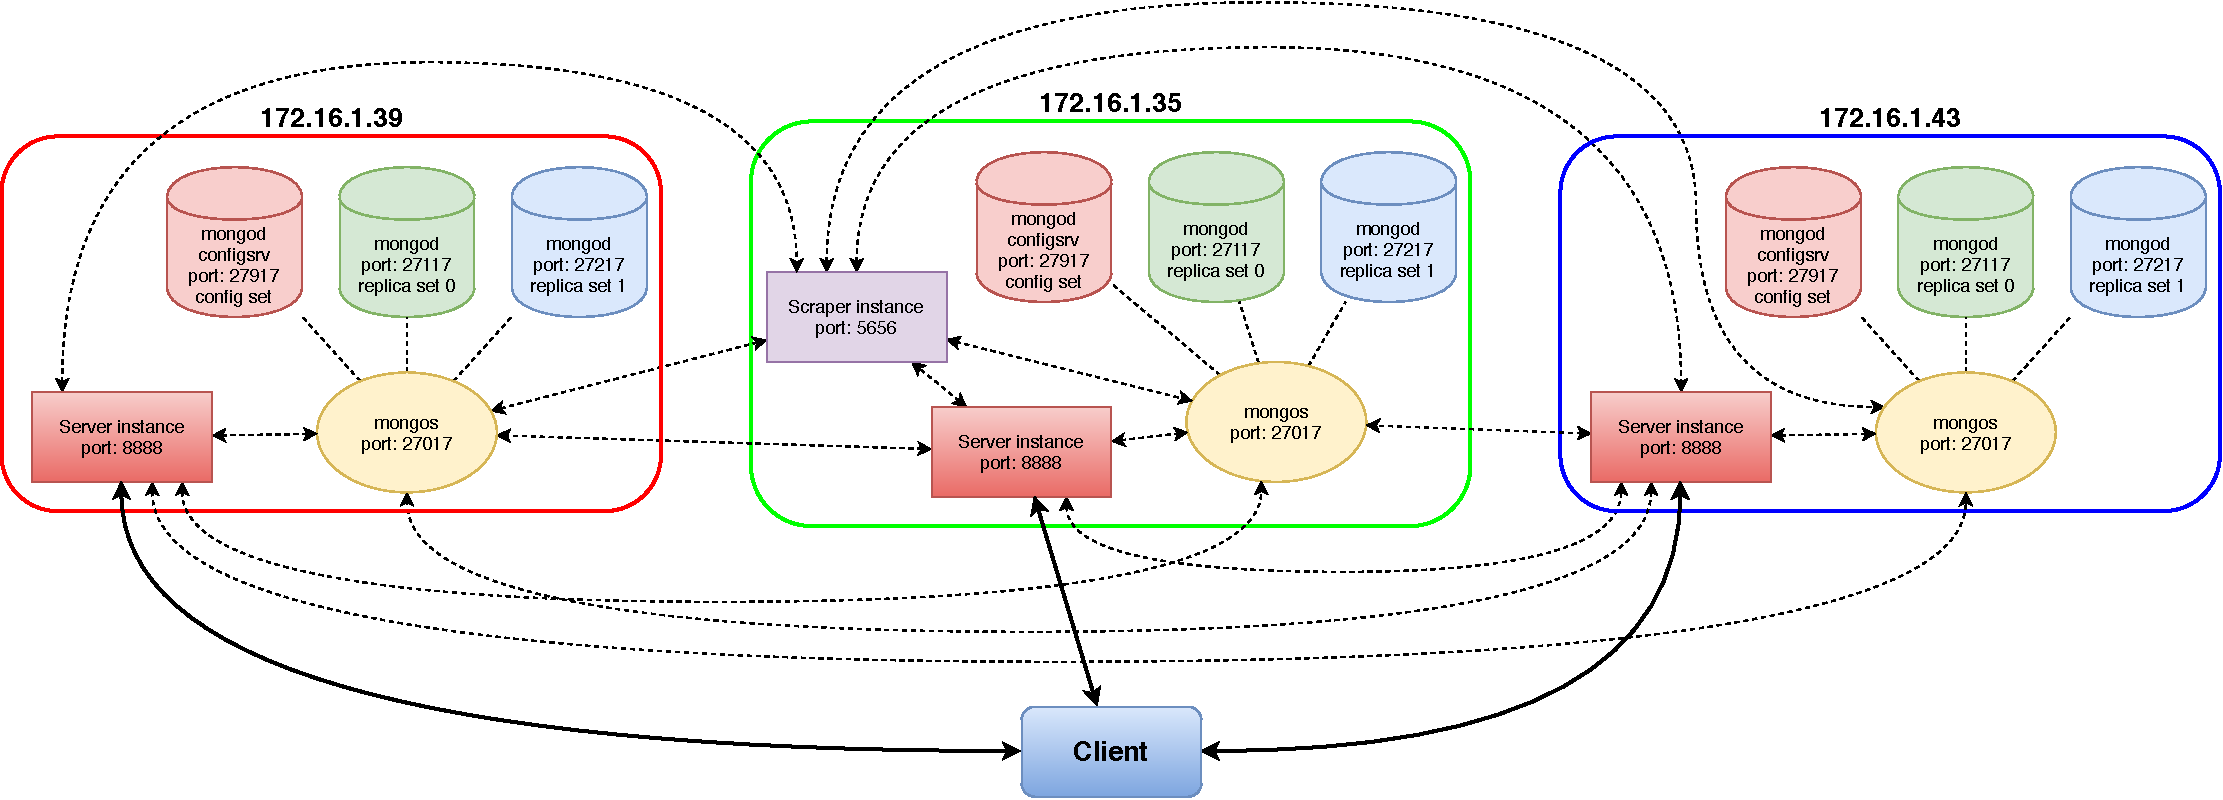
\includegraphics[width=\textwidth]{setup}
	\caption{Application setup on the \theinstitute's
	machines.}\label{fig:setup}
\end{figure}

The \code{/root/strategies} folder is an NFS\footnote{Network File System.}
shared folder. It is shared by \code{172.16.1.35} and mounted on the other two
machines.

If using another configuration, each application has several command line
options to change the connection parameters. You can see all the available
parameters for an application by passing the \code{-h} (\code{--help}) option to
it.

The \code{-c} (\code{--connection-string}) option, available for server and
scraper, allows to change the connection string used to connect to \mongodb.
Here, an example with the default connection string:
\begin{verbatim}
$ java -jar Server.jar -c "mongodb://172.16.1.35:27017,
        172.16.1.39:27017,172.16.1.43:27017"
\end{verbatim}

If \mongodb{} is running as a single standalone instance, you need to pass the
\code{-s} (\code{--standalone}) option to the server and the scraper to disable
the sharding. In this case, server and scraper expect by default to find the
standalone \code{mongod} instance at \code{localhost:27017} (unless changed with
the \code{-c} option).

The server application expect to find the running scraper instance at
\code{172.16.1.35:5656}. If the scraper is running somewhere else, you can use
the server's \code{-H} (\code{--scraper-host}) and \code{-P}
(\code{--scraper-port}) options in order to override the default value.

If multiple instance of the server are running, these must share the directory
where containing the Java classes for the uploaded strategies. This can be done
with NFS if the server instances are running on different hosts. The server's
\code{-D} (\code{--strategies-dir}) option allows to change the directory where
the uploaded strategies will be saved.

The client's \code{-H} (\code{--hosts}) option can be used to set a different
(list of) server(s) to connect to. See \secref{sec:clientrun} for details.

On first start, the server will ask to create the administrator's account.
